\clanguage

\chapter{Description de l'architecture choisie}
\section{Tâche}
La première réflexion apportée concerne les tâches. En effet, il est spécifié que les tâches peuvent être soit unitaire soit préemptive, que les tâches, si elles sont unitaires, peuvent être soit préemptive soit ne pas l’être, et que les tâches composites peuvent contenir des tâches, qui sont à leur tour soit composite soit unitaire. 
Voici un descriptif UML de la solution choisie:

\begin{figure}[h]
	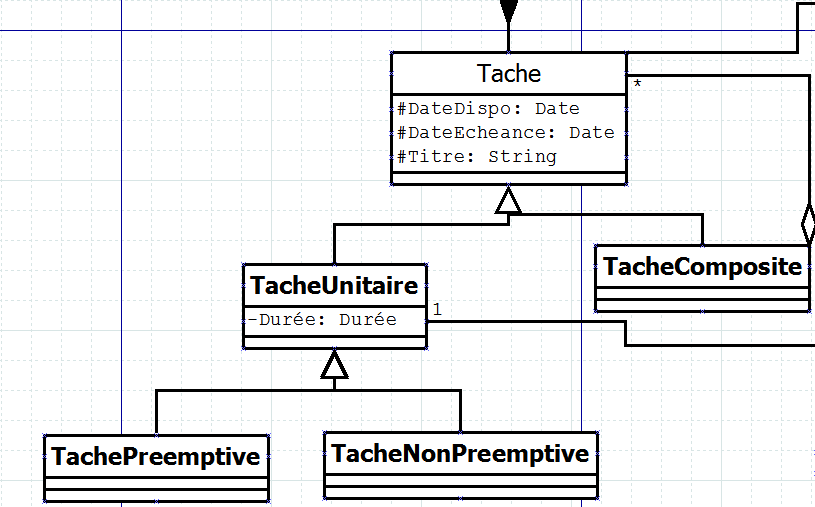
\includegraphics[scale=0.5]{ressources/figure1.png}
\end{figure}

Explications : Nous avons une classe abstraite Tache, que l’on fait spécialiser en TacheUnitaire et TacheComposite. Cette solution, en plus de pouvoir ne spécifier une durée qu’au sein des tâches unitaires, permet aux taches composite de facilement comporter à la fois des sous tâches unitaires et des sous tâches composite en ayant une agrégation avec la classe mère. Nous avons donc là une utilisation du Design Pattern Composite. Le fait d’avoir une classe abstraite tâche permet aussi l’évolutivité du code, car si un jour, un autre type de tâche apparait, il suffira d’hériter de tâche.
Ensuite, nous avons décidé de faire hériter à nouveau TacheUnitaire en TachePréemptive et en TacheNonPreemptive au lieu de simplement mettre un booléen, toujours dans un souci d’évolutivité car il est de se fait plus facile d’avoir des comportements spécifiques à l’un ou à l’autre en ne mettant les fonctions que dans l’un ou dans l’autre par exemple. 

\section{Les programmations}
Ensuite, il a fallu réfléchir aux programmations. Une programmation peut soit porter sur une tâche unitaire, soit porter sur une activité. 
Plusieurs implémentations étaient possibles, comme créer une classe abstraite évènement et en faire hériter tache unitaire et activité, seulement cela comportait le léger inconvénient d’avoir de l’héritage multiple à gérer au niveau de TacheUnitaire, du coup nous avons préféré implémenter une classe abstraite Programmation et d’avoir donc des ProgTUnit et ProgActivite qui en héritent, et qui possèdent chacune un pointeur vers soit la TacheUnitaire, soit l’Activite créée.
\begin{figure}[h]
	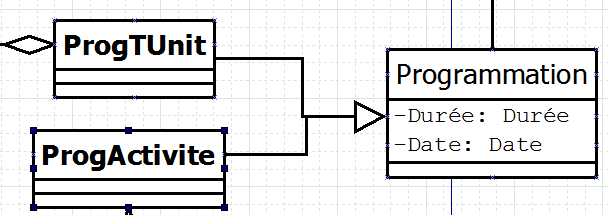
\includegraphics[scale=0.5]{ressources/figure2.png}
\end{figure}

\section{Le manager}
Une fois ceci fait, vient la préoccupation des manager. En effet, afin de pouvoir facilement retrouver et manipuler les différentes entités du programme, il nous fallait des Manager.
Voici leur représentation UML :
\begin{figure}[h]
	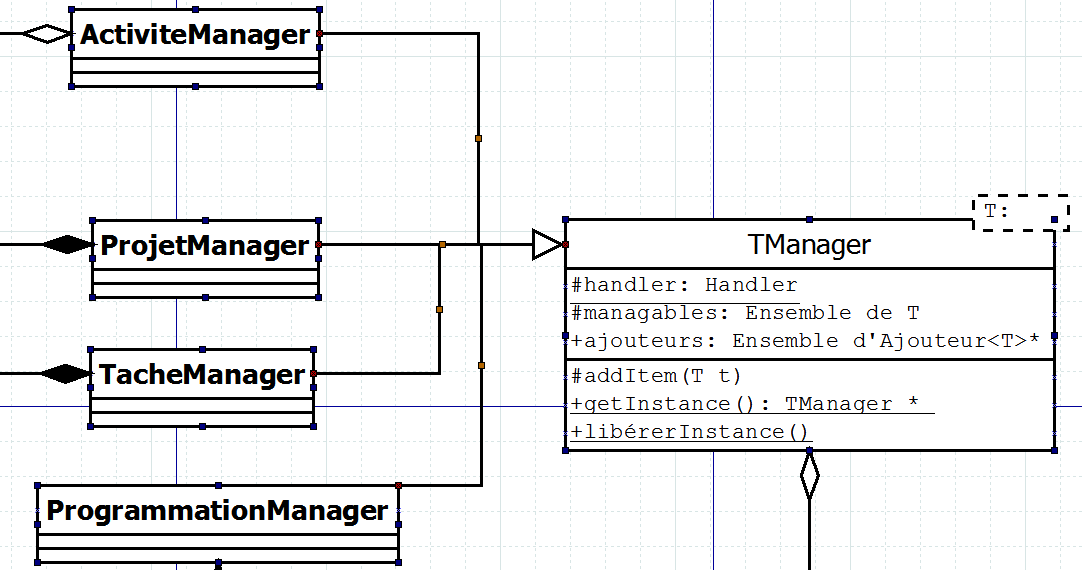
\includegraphics[scale=0.4]{ressources/figure3.png}
\end{figure}

Nous avons donc décidé d’avoir un Manager à la fois comme classe patron et comme singleton. En effet, les manager partagent tous les mêmes fonctionnalités, la seule chose qui les différencie est le type d’objet stocké. Le Manager est singleton car il n’y a besoin que d’une instance de cette classe pour gérer tous les objets qui lui sont associés. Ainsi, en héritant de cette classe patron-singleton, on peut avoir une instance de Manager spécialiser dans le type d’objet voulu. C’est également évolutif car si un jour, il y a un nouveau type d’objet à gérer, il suffira de créer une nouvelle classe qui héritera du manager générique et elle disposera ainsi de l’ensemble des fonctionnalités qui lui sont nécessaires.

\section{Les ajouteurs}
La grosse particularité de notre architecture vient de ses Ajouteurs.
\begin{figure}[h]
	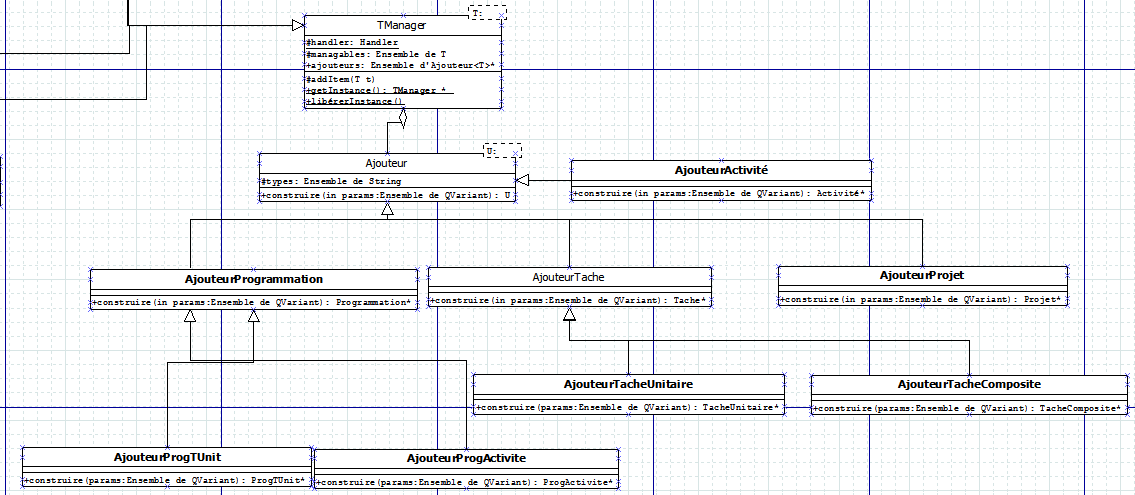
\includegraphics[scale=0.4]{ressources/figure4.png}
\end{figure}
Les Ajouteurs servent à implémenter une architecture très proche de celle du Design Pattern Factory. En effet, les Manager délèguent la création de leurs objets à des ajouteurs. En effet, dans une architecture classique, le TacheManager aurait par exemple la méthode "AjouterTacheUnitaire" ainsi que la méthode "AjouterTacheComposite". Cela pose un problème d’évolutivité, car dans le cas où un nouveau type de tache apparait, il faudrait rajouter une méthode dans le TacheManager, et ainsi recompiler tout le code qui lui est associé. Les Ajouteurs contournent ce problème car en cas de nouvelle tâche, il suffira de créer un Ajouteur associé, et de l’ajouter au Manager grâche à sa méthode "ajouterAjouteur". Leur architecture est basée sur une classe mère patron et un héritage successif selon le type traité.
Cette architecture comportait néanmoins plusieurs difficultés. La première est qu’il fallait que le TacheManager ait accès seulement aux ajouteurs de Taches, le ProjetManager aux ajouteurs de projets etc, et qu’on ne puisse pas s’en servir de l’extérieur, seulement les créer. La solution trouvée consiste à mettre la méthode de création d’objet en privé et de mettre en ami le Manager de même type réel que l’ajouteur, et uniquement celui-ci.
Ensuite, et c’est le problème principal, est que pour pouvoir utiliser efficacement le design pattern factory, il fallait que tous les Ajouteurs possèdent la même fonction de création. Seulement, selon l’objet créé, ils ne possèdent absolument pas les mêmes paramètres. La solution trouvée consiste à utiliser une map liant une chaine de caractère à un QVariant. Un QVariant est un type Qt pouvant se convertir en n’importe quoi à partir du moment où on a averti le compilateur. Ainsi, on peut avoir autant de paramètre que l’on veut du type que l’on veut. Pour s’assurer que l’utilisateur ne rentre pas n’importe quoi, on vérifie que la chaîne de caractère associée au paramètre est bien contenue dans la liste que l’ajouteur possède. 

\section{Exportation}
L'exportation des données semble au premier abord une problématique simple. En effet on pourrait commencer par se dire que pour chaque type d'exportation et chaque format, il suffit de créer une classe spécifique. Cela voudrait dire qu'on aurait, par exemple, une classe pour exporter des programmations en XML, une pour exporter en SQLite, une pour exporter des projets en XML, et ça pour chaque type et format. Nous pourrions nous satisfaire de cette solution mais cela provoquerai de la duplication de code d'une part, et une évolutivité restreinte. Si je souhaite exporter mes programmations dans un format quelconque, je serais obliger de recoder totalement l'algorithme d'exportation. C'est en souhaitant palier à ces défauts que nous avons choisi une architecture basée sur le design pattern strategy, qui sera d'ailleurs appliqué deux fois dans cette architecture.
Le principe est de découper l'exportation en deux parties (figure \ref{Annexe2}):
\begin{itemize}
    \item Une partie concernant le type d'exportation (Programmations, Projets, ect...), qui contiendra l'algorithme général d'exportation.
    \item Une partie concernant les formats d'exportation (XML,SQLite,Fichier,ect...) qui possèdera les méthodes de formatage des données.
\end{itemize}
\subsection{Les types d'exportation et le template TExport}
Cette partie de l'architecture est une architecture en trois niveaux:
\begin{itemize}
	\item Le template \textbf{TExport} permettant de définir la structure général des classes d'exportation.
	\item Une classe abstraite héritant de ce template permettant de définir le type d'exportation à effectuer, ici par exemple \textbf{ProgrammationExport} qui permet d'exporter des programmations. Cette classe doit définir la méthode \textbf{exportData()} qui est la structure générale de l'exportation. Dans le cas des programmations par exemple, on définit qu'il va falloir récupérer les tâches, les projets liés à ces tâches, et récupérer les activités.
	\item Une classe concrète définissant plus finement ce que l'on veut exporter. Par exemple la classe \textbf{ProgrammationSemaineExport} se charge des programmations d'une semaine particulière, tandis que \textbf{ProgrammationProjetExport} se charge des programmations relatives à un projet. La différence entre les deux classes se joue sur la récupération des programmations, définie grâce à la méthode \textbf{findElements()}.
\end{itemize}
\subsection{Les différents formats d'exportation}
Nous avons choisi d'utiliser un pattern Strategy afin d'associer type d'exportation et format de telle sorte à rendre modulable l'utilisation. Ainsi cette seconde partie consiste également en une classe généralisant toutes les autres et indiquant les méthodes à implémenter afin de rendre fonctionnel l'exportation. Ici nous avons donc une classe \textbf{MethodExport}, abstraite, avec comme attribut une extension, correspondant à l'extension du fichier final, et une méthode d'exportation par élément à exporter, c'est-à-dire une méthode pour exporter un projet, une pour exporter une tâche, une pour exporter une programmation et une pour exporter une activité. Nous avons ensuite une fonction sendExport qui va permettre de transformer le formatage en la chaine de caractère qui sera insérée dans le fichier dans la première partie.
Définir un type d'exportation devient donc relativement simple: il suffit d'étendre la classe MethodExport et d'implémenter ces 5 méthodes.
\subsection{Facilité d'évolution}
L'architecture choisies permet d'adapter facilement en cas d'évolution. Si nous souhaitons ajouter un nouveau type d'exportation (par exemple exporter des projets), il suffira d'étendre la classe TExport et de définir comment exporter. Si nous souhaitons exporter dans un nouveau format, c'est du côté de la classe MethodExport qu'il faudra se diriger, l'étendre et définir les méthodes de formatage des éléments.